\section{Implementation}

\subsection{Code overview}

\begin{figure}[h!]
    \centering
    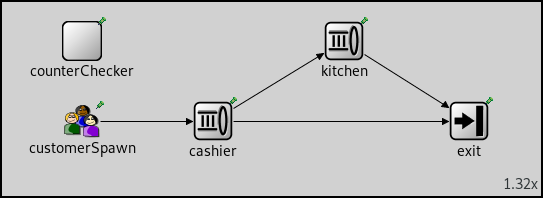
\includegraphics[width=.75\textwidth]{figs/omnet_network.png}
    \caption{Diagram of the Omnet++ network.}
    \label{fig:omnet_network}
\end{figure}

The Omnet++ network is composed of 5 nodes:
\begin{itemize}
    \item \textbf{customerSpawn}: generates the orders using a configurable
        distribution.
    \item \textbf{cashier}: serves orders and, upon completion, sends them to 
        the \emph{kitchen} if they are compound or to the \emph{exit} otherwise.
        The type of order is determined in the \emph{customerSpawn} node.
    \item \textbf{kitchen}: serves orders and sends them to the \emph{kitchen}
        upon completion.
    \item \textbf{exit}: collects statistics about order response times and 
        disposes of them.
    \item \textbf{counterChecker}: collects number of generated, exited and 
        in-queue orders in order to check that no order is lost.
\end{itemize}

% \subsection{Verification}

% \subsubsection{Debugging}

\subsubsection{Validation}
In order to verify that the implementation exaclty reflects our model, we 
carried out the following tests.

\paragraph{Test 1: Single-type orders with constant inter-arrival times}
Only orders of a single type are generated with constant inter-arrival times
in order to check that the correct path is followed by the orders and that 
statistics collection is working correctly. 
Note that in this case there is no queueing.

\paragraph{Test 2: Simple and compound normal orders with constant inter-arrival times}
Only normal orders are generated, both simple and compound, with constant inter-arrival times
in order to check that the orders are correctly routed between kitchen and exit with 
the set probability.

\paragraph{Test 3: Normal and VIP simple orders with constant inter-arrival times}
Only simple orders are generated, both normal and VIP, with constant inter-arrival times
in order to check that the priority queueing works correctly. In order to do that, 
two normal orders are sent at time t=1 and t=2 respectively, a VIP order is sent 
at time t=2.5 and the service time is 2. It is expected the last VIP order to be 
serviced second.

\paragraph{Test 3b: Normal and VIP compound orders with constant inter-arrival times}
Only compound orders are generated, both normal and VIP, with constant inter-arrival times
in order to check that the priority queueing works correctly. In order to do that, 
two normal orders are sent at time t=1 and t=2 respectively, a VIP order is sent 
at time t=2.5 and the service time is 2. It is expected the last VIP order to be 
serviced second. The test is repeated for both FIFO and priority queue in the kitchen.

\paragraph{Test 4: Simple orders with exponential inter-arrival times}
Simple orders are generated with exponential inter-arrival times and the 
mean response time for each kind is compared with the mathematical model. Several 
scenarios are considered namely:
\begin{itemize}
    \item total arrival rate is kept constant to 1 while the proportion of 
        normal and VIP orders varies from 0\% to 100\%, with a step of 25\%.
    \item cashier service rate is varied from $1.1$ to $2$ with a step of $0.1$.
\end{itemize}

\paragraph{Test 4b: Compound orders with exponential inter-arrival times}
Compound and simple orders are generated with exponential inter-arrival times.
Compound orders are $10\%$ of the total, while simple orders are ignored (they are
only generated in order to create a realistic scenario). The 
mean response time for each kind of compound orders is compared with the mathematical 
model. Several scenarios are considered namely:
\begin{itemize}
    \item total arrival rate is kept constant to 1 while the proportion of 
        normal and VIP orders varies from 0\% to 100\%, with a step of 25\%.
    \item kitchen service rate is varied from $0.15$ to $0.5$ with a step of $0.05$.
    \item cashier service rate is kept constant to $1.5$.
\end{itemize}
The test is repeated for both FIFO and priority queue in the kitchen. In the case 
of the priority queue, the mathematical model could not be used so it was checked 
that:
\begin{itemize}
    \item mean response time for normal orders is higher than VIP orders.
    \item mean waiting time for normal orders is higher than VIP orders.
    \item performance indexes are in a continuous relationship with the simulation
        factors.
\end{itemize}

\paragraph{Validation results}
All the validation tests listed above have been passed by the implementation.
Test 4/4b have been checked by automatically plotting, through a script,
the performance metrics. \cref{fig:validation} shows an example of the plots.
You can check all the plots in \texttt{simulation/jupyter/Test.ipynb}.

\begin{figure}[]
    \centering
    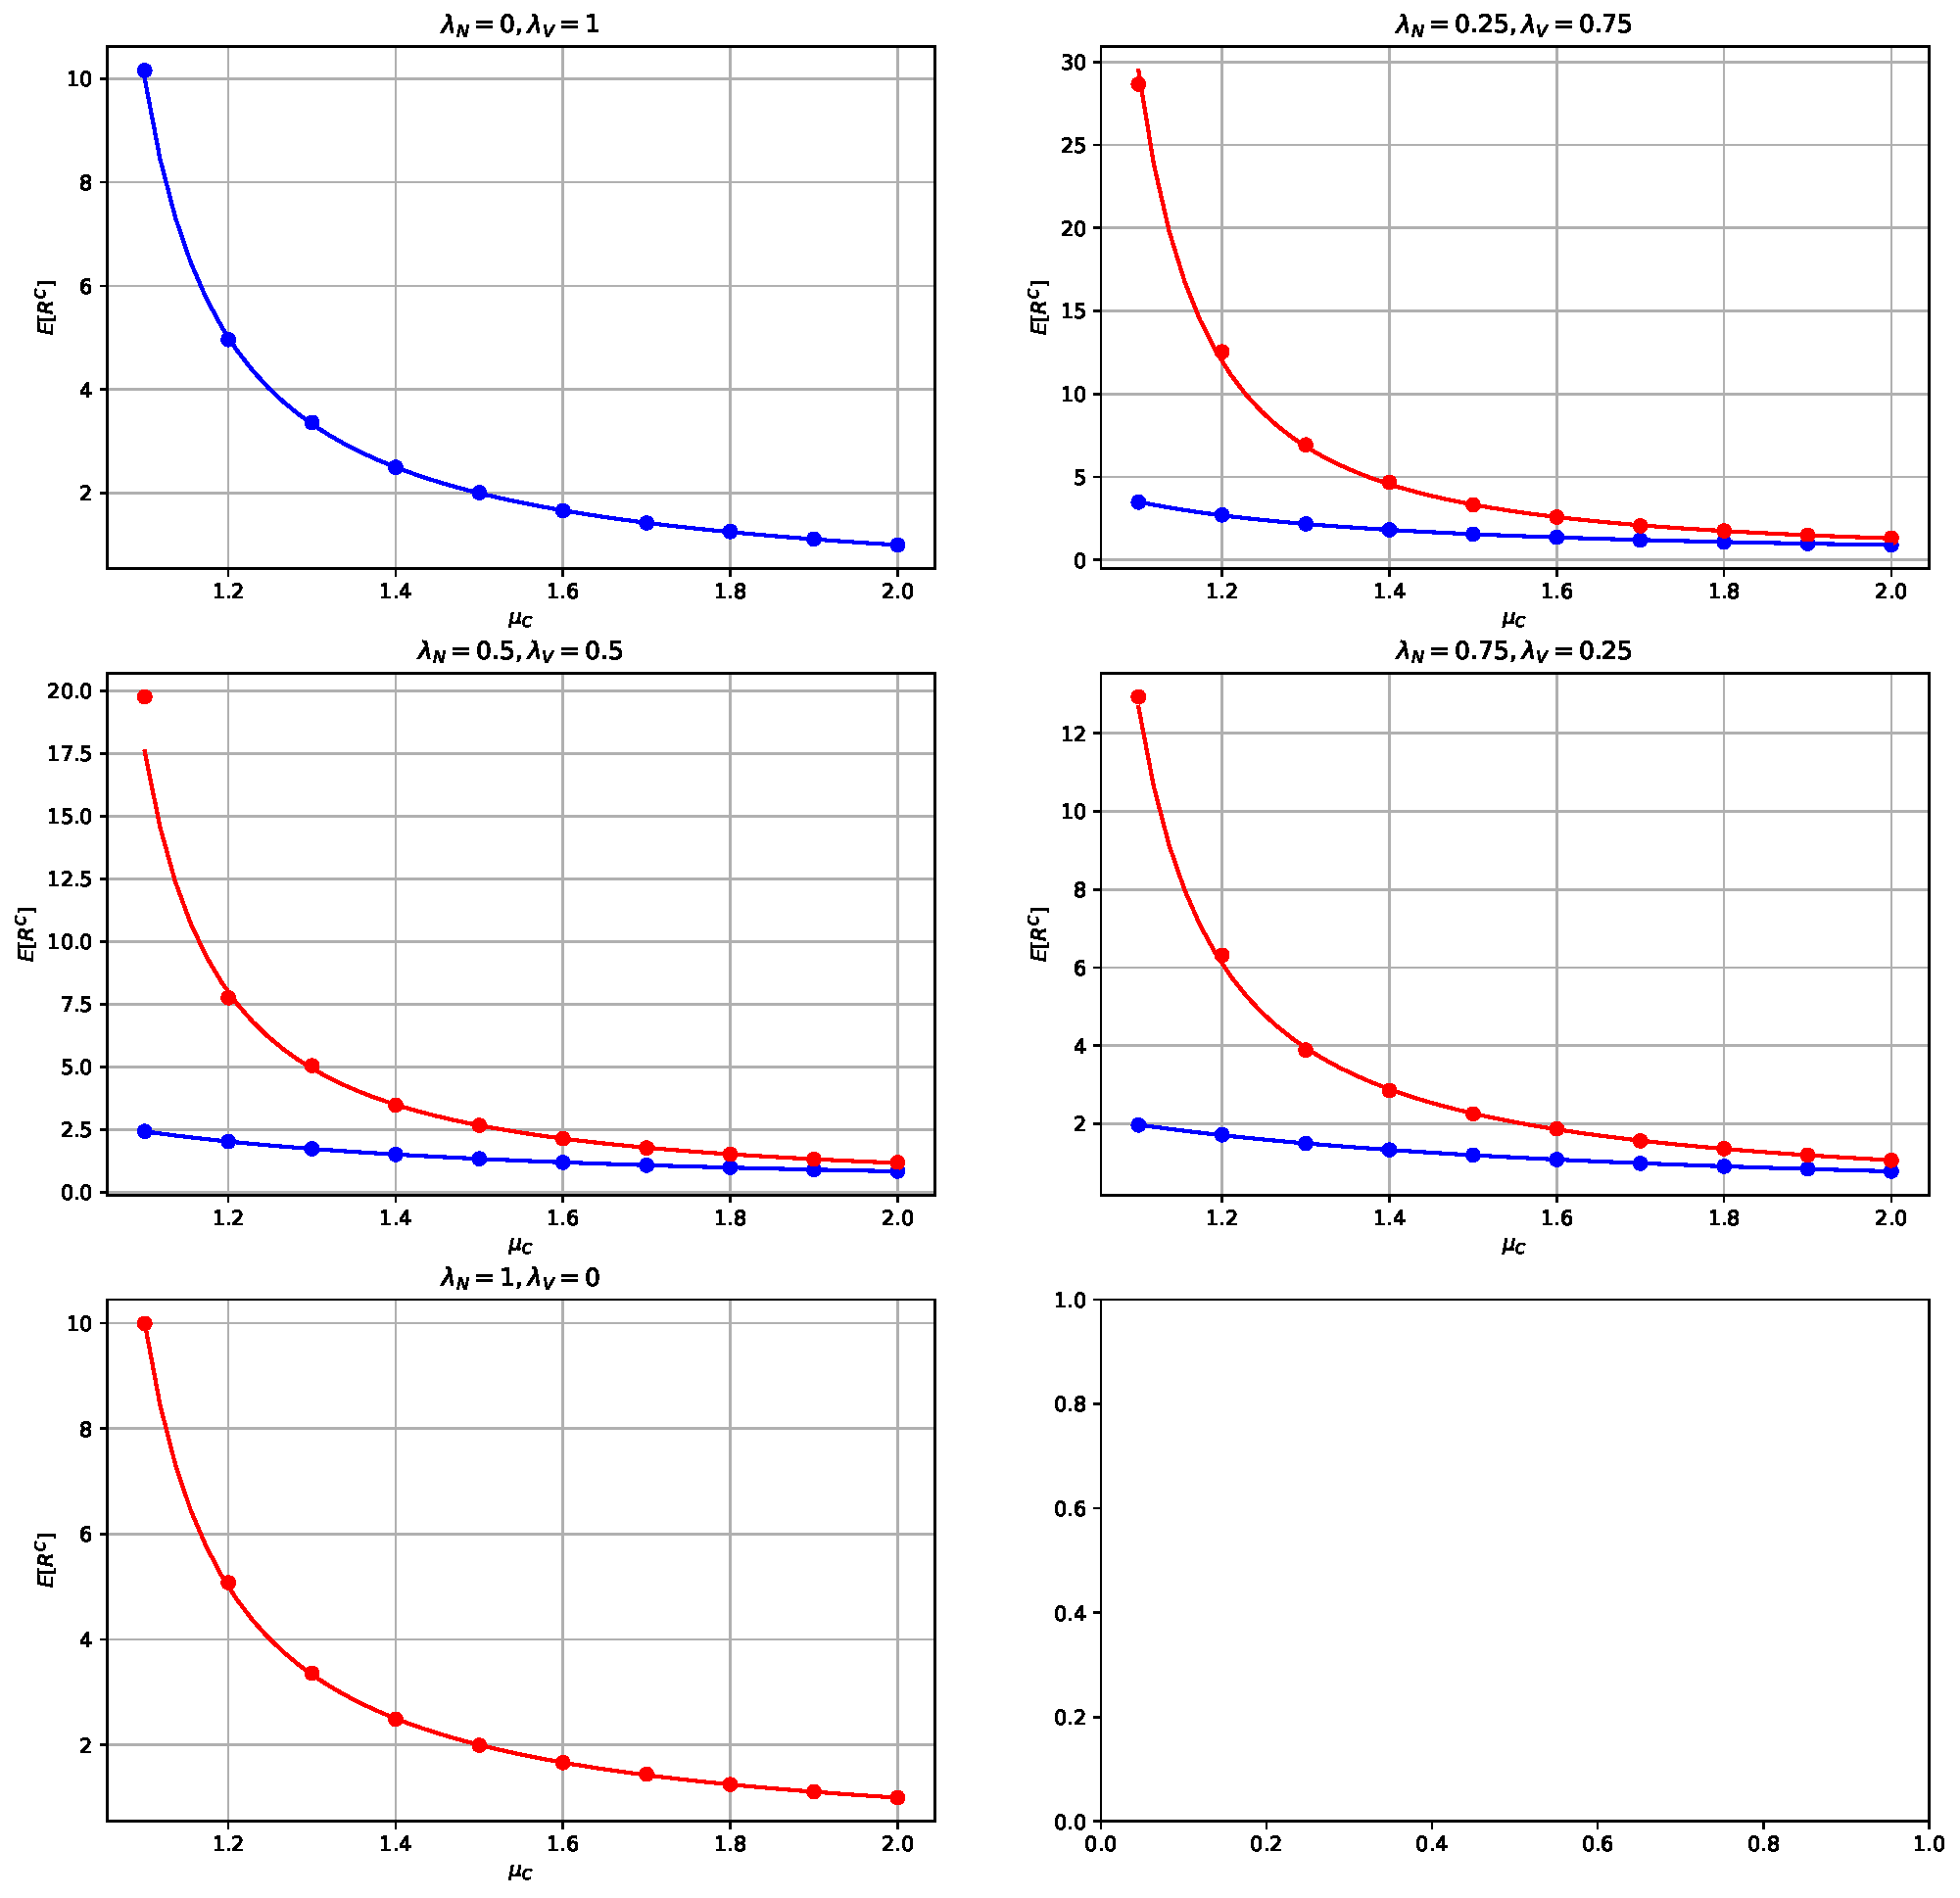
\includegraphics[width=\textwidth]{figs/validation.pdf}
    \caption{Validation of Test 4 showing the mean cashier response time for 
        both VIP (in blue) and normal (in red) customers.}
    \label{fig:validation}
\end{figure}

\subsection{Calibration}
% TODO write used parameters